\chapter{Introduction}\label{ch:introduction}
% Achieving intelligence requires modeling the real world,
% this is true in the context of scientific research but also of engineering tools.
Ever since the beginning of their existence, humans have always been curious to understand the complexity of the world they live in.
This is not only true at the individual level as we keep building and improving our knowledge over our lifespan,
but also at the level of humankind where knowledge has never really stopped rising since the beginning of civilization.
Science, as an objectification of our curiousity, aims at grounding the construction of this common knowledge on rationality. In particular, the modern scientific method
arguably relies on 5 pillars as depicted in \Cref{fig:ch01:scientific_method} which ensure discoveries are made out of rigor and on the basis of current scientific knowledge.
Although the scientific method can answer questions in the context of a specified model of the world as stated by the hypotheses, the more fundamental goal of science is to refine these models by critisizing their ability to predict the real world. In this context, the aim of this thesis is to explore and contribute to modern techniques for building or refining models of the world.
% This thesis is about this: How can we automatically combine scientific knowledge and data to create faithful and useful models?
\begin{figure}[h]
  \centering
  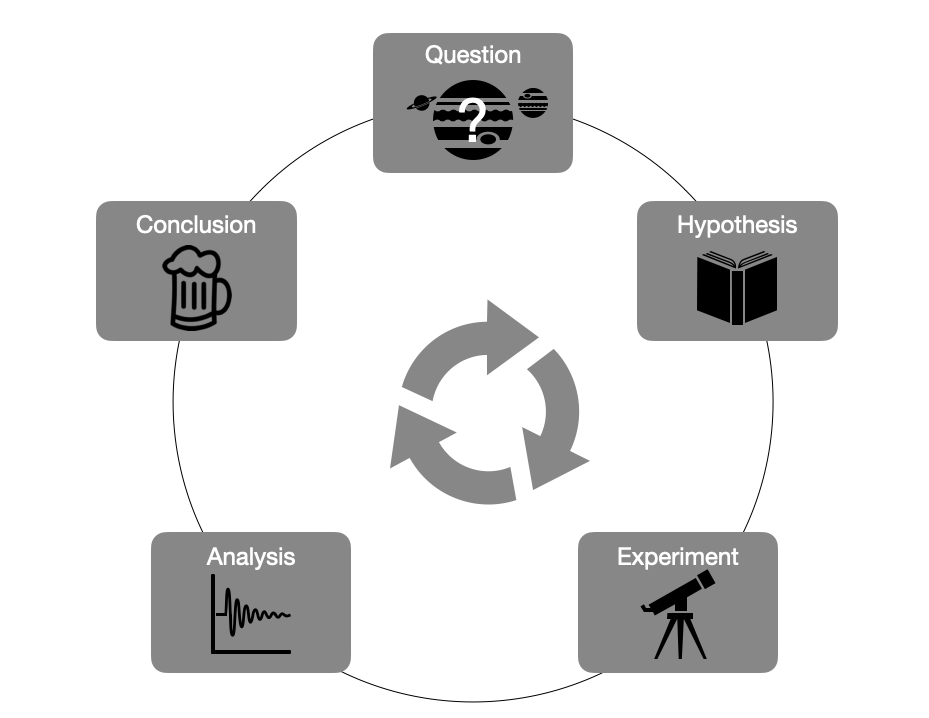
\includegraphics[width=.8\textwidth]{figures/chapter01/trapist_disco.png}
  \caption{Illustration of the scientific inquiry as a simplified 5-steps process.
  The pictograms sketch a cartoon of the TRAPPIST-1 planetary system discovery made by astronomers from Li{\`e}ge university in 2016 \citep{gillon2017seven}.
  A scientist first formulates a \textit{research question} and a set of reasonable \textit{hypotheses}, together they define a class of hypothetical models of the world.
  In order to answer his question, he gathers data from \textit{experiments} and analyze them in the context of his modeling assumptions. Checking the consistency of diffent hypothetical models allows him \textit{to provide an answer} to his initial question up to a certain degree of certainty.}
  \label{fig:ch01:scientific_method}
\end{figure}

Classically, scientists or engineers use their domain expertise to build incrementally complex models and improve their faithfulness to reality. The scientific method then applied validate or reject the new class of models.
This strategy has not only led to today's state of science but also to the uttermost engineering accomplishments of modern times.
In engineering, these successes impact our daily life such as by enabling nuclear electricity - as predicted by special relativity - or
allowing ones to read this manuscript on a smart tablet - thanks to Maxwell equations' implications on the design of modern computers.
More abstract but arguably as impactful on our vision of the universe, the classical model refinment strategy led to all modern scientific breakthroughs. As examples, these models allow astronomers to observe the furthest human-known objects, thanks to general relativity and gravitational lensing, and enable the indirect observations of black holes thanks to gravitational waves theory.


Despite these numerous achievements, the classical modelling approach has recently been challenged by machine learning. Where humans fall short to find patterns in large amount of data and to build arbitrarily complex models, machines can perform these tasks automatically days and nights.
The shift from hand-crafted to automated modeling happens in a world where the most ambitious scientific experiments generate petabytes ($10^{15}$) of data per seconds \citep{noauthor_cern_nodate}. On the one hand, while the computing capacity continuously increases, the human brain is not better wired to aprehend vast amount of data than it was when Galileo Galilei sets the basis of modern science, 400 years ago. On the other hand, deep learning has recently proven its ability to build accurate generative models that outperform the ones designed out of human expertise. This is for example true in the context of voice synthesis \citep{van_den_oord_wavenet_2016}, text-translation \citep{GPT3, bert...}, chat bots, or even text-to-image synthesis \citep{Dall-e-2, imagen}, to cite a few. Under these cirumstances, the paradigm shift, even in a scientific context, seems natural.

Sounds, text, images, all these successes correspond to data modalities that are broadly available. This hints deep generative models are able to process and create a good representation of large datasets. It is especially hard to quantify if these models really understand the structure in the data or they are smart copycats. As an example it is not always easy to ensure that these models do not collapse to a subset of the modes present in the data. Depending on the aim of the model mode collapse can be problematic, e.g. if we want to carefully handle inherent stochasticity observed in the data. In addition, recent works argue that these large models do overfit the training data \citep{overfit_dalle, gpt3}.
This makes sense as there is no reason that would help a neural network to know something it has not seen during training. This may preclude the application of deep generative models in contexts where data are scarcer or if we aim for a model that has a profound understanding of the phenomenon it is trained to represent.
% A partial solution to this problem would be to allow these models to use efficiently the prior knowledge we can have of the modeled process, this is maybe fine when the goal is to do image synthesis but is not when we need a model that satisfies the laws of physics.
% Paragraph on the challenges faced by deep generative models: Trainign difficulty, generalization, consistency with law of physics, interpretability.


\begin{side_note}{Explicit vs. implicit models}
  In general, faithful modeling requires to account for uncertainty. This is important as, by definition, models are simplified representation of the reality and so cannot explicitly represent all possible sources of pertubations deterministically. As an example the precision of any sensor is determined by fitting a model that accounts stochasticaly for internal and external perturbation that may arise in practical setting such as the temperature, humidity or pressure. This is of course true for small models that are usually simplistic but also for larger models that builds on top of smaller stochastic models. These models define stochastic generative processes that synthesize observations $\mathbf{x}$ conditionally on the models' parameters $\mathbf{\theta}$. When it comes to the classical approach, the complexity of the models depends on the granularity of the different effects taken into account. And while small models simply corresponds to simple statistical assumptions and provide access to the likelihood function $p(\mathbf{x}|\mathbf{\theta})$, larger models are computer programs for which the likelihood is usually intractable because of the multiple sources of randomness. We use the terms \textit{explicit} and \textit{implicit} to distinguish between models that provide \textit{explicit} access to the likelihood function and those that do not. The same distinction goes for deep generative models that can either provide access to the likelihood or only generative process.
\end{side_note}
\section{Research question}
Motivated by this paradigm shift and the remaining challenges in deep generative modeling, this thesis contributes to answering the following reseach question:
\begin{center}
  \textit{How can we improve the construction of faithful generative models with deep learning algorithms?}
\end{center}
In the pursuit of this objective we explore several directions that study and improve on different aspects of deep generative models. In particular, we make the distinction between data-driven models that only rely on the inductive bias of the learning algotithms and the availability of representative data, and hybrid models that embed strong prior knowledge (e.g. independence assumptions or partial understanding of the underlying physics) into deep generative models. We argue that contributions to both aspects are complementary and will improve the range of application of deep generative models. On the one hand, data-driven algorithms are well suited to modeling tasks for which we do not have strong domain knowledge but access to a lot of representative data. On the other hand, hybrid modeling allows the combination of domain knowledge with data and is thus better equipped against small or poorly representative datasets.
% A word somewhere that scientific models are usually probabilistic generative models because good models require modeling uncertainty coming from unmodeled phenomenon or phenomenon
% that are only modeled up to a certain level of stochasticity. Introduced the concept of explicit generative vs implicit generative models

% Paragraph arguing that we still need to work on deep generative models as they are not perfect yet.


% Even granted with perfect optimization procedures and universal generative models, the problem would not be solved. To fight the curse of dimensionality
% we need strong inductive bias. But more than the curse of dimensionality we also often requires these models to not stupidly fall as soon as they are required to
% act in an environment slightly different from the training configuration. We want these models to be able to built on current knowledge. It may also be important that these Models
% have a level of interpretability for humans especially if we want to use them in a scientific context. The second part of this thesis study this equally important aspect.


\section{Outline and structure}


Before diving into the core contributions of this thesis, a review of probabilistic modeling in \Cref{ch:02} naturally follows this introduction and provide all notions necessary to the appreciations of this thesis for a reader equiped with a technical background. Then, \Cref{part:1} focuses on improving the expressivity and learning algorithms of implicit and explicit deep generative models. To this end, we explore two independent directions respecively on implicit and explicit generative models. First, \Cref{ch:03} studies the complementarity of two classes of implicit generative models, namely the variational auto-encoders and the diffusion models, and show that diffusion models are a good replacement to the simple Gaussian distributions classicaly used to model a prior over the latent variables of variational auto-encoders. We then start our exploration of explicit generative models in \Cref{ch:04} by showing that affine normalizing flows, a class of explicit models, are unable to represent arbitrary generative models. The first part ends in \Cref{ch:05} that addresses the expressivity issues of affine normalizing flows by introducing a new neural architecture to model monotonic functions. \Cref{part:2} explores hybrid modeling, a class of models that embrace the opportunity to combine pre-existing domain knowledge within deep generative models. In particular, \Cref{ch:06} studies the modeling and implications of independence assumptions in normalizing flows while \Cref{ch:07} studies the generalization capabilities of deep generative models equipped with a partial model of the studied process. As a conclusion and summary, \Cref{ch:08} reflects upon the contributions of this thesis and current challenges faced by deep generative models.



% Paragraph Arguing generative models are not data efficient because they do not built on common knowledge as would do a human

% Historically modeling was achieved by manually describing sub-part of the studied processed with simple physical equations.
% Machine learning led to a paradigm shift in this context.

% The aim of this thesis is to study and improve generative modeling in this context (paradigm shift from hand crafted to automated modeling).
% Two aspects of improments are proposed
% 1) Improving and studying the expressivity of automated probabilistic modeling approaches.
% 2) Combining domain knowledge with data driven approaches to achieve faithful and generalizable modeling.
% Both aspects are as important as on the one hand the availability of data increases for many problems which opens the path to breakthrough in the modeling of complex phenomenon.
% On the second hand, data are usually biased in some sense and generalization outside of this can only happen by enforcing invariance or equivariance with respect to spme aspects of the problems or real world.


\section{Publications}
Setting aside this introduction, an original primer on probabilistic modeling in \chapref{02} and the conclusion,
the scientific content of this manuscript is exclusively borrowed to original contributions made to generative modeling over the last 4 years.
Each selected contribution sets its own chapter complemented with a prologue and an epilogue.
The manuscript builds upon the following list of publications:

\begin{tcolorbox}[width=\textwidth,colback={grey},title={List of publications},outer arc=0mm,coltitle=white]

  \begin{itemize}
  \item[] \citep{wehenkel_unconstrained_2019} \textit{Unconstrained monotonic neural networks},
  \textbf{Wehenkel Antoine} and Louppe Gilles.\\
  Advances in neural information processing systems, 2019.\\
  $\quad \rightarrow$ \chapref{05}.

  \item[] \citep{wehenkel_you_2020} \textit{You say Normalizing Flows I see Bayesian Networks},
  \textbf{Wehenkel Antoine} and Louppe Gilles.\\
  International Conference on Machine Learning, Workshop on Invertible Neural Networks, Normalizing Flows, and Explicit Likelihood Models, 2020.\\
  $\quad \rightarrow$ \chapref{04}.

  \item[] \citep{wehenkel2021graphical} \textit{Graphical Normalizing Flows},
  \textbf{Wehenkel Antoine} and Louppe Gilles.\\
  International Conference on Artificial Intelligence and Statistics, 2021.\\
  $\quad \rightarrow$ \chapref{06}.

  \item[] \citep{wehenkel2021diffusion} \textit{Diffusion Priors In Variational Autoencoders},
  \textbf{Wehenkel Antoine} and Louppe Gilles.\\
  International Conference on Machine Learning, Workshop on Invertible Neural Networks, Normalizing Flows, and Explicit Likelihood Models, 2021.\\
  $\quad \rightarrow$ \chapref{03}.

  \item[] \citep{wehenkel2022robust} \textit{Robust Hybrid Learning With Expert Augmentation},
  \textbf{Wehenkel Antoine}, Behrmann Jens, Hsu Hsiang, Sapiro Guillermo, Louppe Gilles, and Jacobsen J{\"o}rn-Henrik.\\
  In preparation, arXiv preprint arXiv:2202.03881.\\
  $\quad \rightarrow$ \chapref{07}.

  \end{itemize}
\end{tcolorbox}


Along the pursuit of my PhD degree, I had the chance to take part in fruitful collaborations not directly related to the scope of this thesis.
The following list of co-authored publications stemmed from these collaborations:

\begin{tcolorbox}[breakable,width=\textwidth,colback={grey},title={Extra contributions},outer arc=0mm,coltitle=white]

\begin{itemize}
\item[] \citep{pesah2018recurrent} \textit{Recurrent Machines For Likelihood-free Inference},
Arthur Pesah, \textbf{Wehenkel Antoine} and Louppe Gilles.\\
Advances in neural information processing systems, MetaLearn Workshop, 2018.

\item[] \citep{wehenkel2020parameter} \textit{Parameter Estimation Of Three-phase Untransposed Short Transmission Lines From Synchrophasor Measurements},
\textbf{Wehenkel Antoine}, Mukhopadhyay Arpan, Le Boudec Jean-Yves, Paolone Mario.\\
IEEE Transactions on Instrumentation and Measurement, 2020.

\item[] \citep{vecoven2020introducing} \textit{Introducing Neuromodulation In Deep Neural Networks To Learn Adaptive Behaviours},
Vecoven Nicolas, Ernst Damien, \textbf{Wehenkel Antoine}, Drion Guillaume.\\
PloS one 15 (1), e0227922.

\item[] \citep{vandegar2021neural} \textit{Neural Empirical Bayes: Source Distribution Estimation and its Applications to Simulation-Based Inference},
Vandegar Maxime, Kagan Michael, \textbf{Wehenkel Antoine} and Louppe Gilles.\\
International Conference on Artificial Intelligence and Statistics, 2021.

\item[] \citep{delaunoy2020lightning} \textit{Lightning-Fast Gravitational Wave Parameter Inference through Neural Amortization},
Delaunoy Arnaud, \textbf{Wehenkel Antoine}, Hinderer Tanja, Nissanke Samaya, Weniger Christoph, Williamson Andrew R and Louppe Gilles.\\
Advances in neural information processing systems, ML4Science Workshop, 2020.

\item[] \citep{hermans2021averting} \textit{Averting A Crisis In Simulation-based Inference},
Hermans Joeri, Delaunoy Arnaud, Rozet Fran{\c{c}}ois, \textbf{Wehenkel Antoine} and Louppe Gilles.\\
In preparation, arXiv preprint arXiv:2110.06581.

\item[] \citep{dumas2021probabilistic} \textit{A Probabilistic Forecast-driven Strategy For A Risk-aware Participation In The Capacity Firming Market},
Dumas Jonathan, Cointe Colin, \textbf{Wehenkel Antoine}, Sutera Antonio, Fettweis Xavier and Corn{\'e}lusse Bertrand.\\
IEEE Transactions on Sustainable Energy, 2021.

\item[] \citep{dumas2022deep} \textit{A Deep Generative Model For Probabilistic Energy Forecasting In Power Systems: Normalizing Flows},
Dumas Jonathan, \textbf{Wehenkel Antoine}, Lanaspeze Damien, Corn{\'e}lusse Bertrand and Sutera Antonio.\\
Applied Energy, 2022.

\end{itemize}
\end{tcolorbox}
